\documentclass[11pt]{article}

\usepackage{deauthor,times,graphicx}

% JobGraph fig
\usepackage{tikz}
\usetikzlibrary{arrows,automata,positioning,shapes.geometric}

% trademark symbol
\usepackage{textcomp}

\usepackage{float}


\newcommand{\TODO}[1]{\textcolor{red}{TODO: #1}}

% code listings
\usepackage{listings}

\newcommand{\sectionautorefname}{Section}%

\newcommand{\para}[1]{\vspace{2mm}\noindent\textbf{#1}}

\definecolor{dkgreen}{rgb}{0,0.6,0}
\definecolor{gray}{rgb}{0.5,0.5,0.5}
\definecolor{mauve}{rgb}{0.58,0,0.82}

% there is no built in support or Scala yet, good enough
\lstset{frame=l,
  language=Java,
  aboveskip=3mm,
  belowskip=3mm,
  showstringspaces=false,
  xleftmargin=5pt,
%   framexleftmargin=-1pt,
  columns=flexible,
  basicstyle={\scriptsize\ttfamily},
  numbers=none,
  numberstyle=\tiny\color{black},
  keywordstyle=\color{blue},
  commentstyle=\color{dkgreen},
  stringstyle=\color{mauve},
  breaklines=true,
  breakatwhitespace=true,
  tabsize=4,
  %for scala
  emph={%  
    object, def, val, zip, window, trigger, evict%
    },emphstyle={\color{blue}\textbf}%
}%

% url references
\usepackage{hyperref}

% in paragraph enums
\usepackage{paralist}

\usepackage{subfigure}

\def\definitionautorefname{Definition}
\def\sectionautorefname{Section}
\def\subsectionautorefname{Section}
\def\subsubsectionautorefname{Section}
\def\algorithmautorefname{Algorithm}
\def\figureautorefname{Figure}

\begin{document}

\title{Apache Flink\texttrademark: Unified Stream and Batch Processing \\ in a Single Engine}

\author{Authors}

\maketitle

\begin{abstract}
Apache Flink is an open source system for processing streaming and batch data. Flink is built on the philosophy that many classes of data processing applications, including real-time analytics, continuous data pipelines, historic data processing (batch), and iterative algorithms (machine learning, graph analysis) can be expressed and executed as pipelined fault tolerant dataflows. In this paper, we present Flink’s architecture and expand on how a (seemingly diverse) set of use cases can be unified under the same execution model.
\end{abstract}

%!TEX root = paper.tex


\section{Introduction}
\label{sec:intro}
Data stream processing (e.g, as exemplified by Complex Event Processing systems) and static (batch) data processing (e.g., as exemplified by MPP databases and Hadoop ) were traditionally considered as two very different types of applications. They were programmed using different programming models and APIs, and were executed by different systems (for example, dedicated streaming systems such as  Apache Storm, IBM Infosphere Streams, Microsoft Streaminsight, or Streambase versus relational databases or execution engines for Hadoop, including Apache Spark, Apache Drill, etc). Traditionally, batch data analysis made up for the lion share of the use cases, data sizes, and market, while streaming data analysis mostly served specialized applications.

It is becoming more and more apparent, however, that a huge number of today's large scale data processing use cases handle data that is, in reality, continuously produced over time. These continuous streams of data come for example from web logs, application logs, sensors, or as changes to application state in databases (transaction log records). Rather than treating the streams as streams, today's setups ignore the continuous and timely nature of data production. Instead, data records are (often artificially) batched into static data sets (for example hourly/daily/monthly chunks) and then processed in a time-agnostic fashion. Data collection tools, workflow managers, and schedulers orchestrate the creation and processing of batches, in what is actually a continuous data processing pipeline. Architectural patterns like the "lambda architecture" \cite{marz2015big} combine batch and stream processing systems to implement multiple paths of computation: A streaming fast path for timely approximate results, and a batch offline path for late accurate results. All these approaches suffer from high latency (imposed by batches), high complexity (connecting and orchestrating several systems, and implementing business logic twice), as well as arbitrary inaccuracy, as the time dimension is not explicitly handled by the application code.

Apache Flink follows a paradigm that embraces data stream processing as the unifying model for real-time analysis, continuous streams, and batch processing, both in the programming model and in the execution engine. In combination with durable message queues that allow quasi arbitrary replay of data streams (like Apache Kafka\footnote{http://kafka.apache.org/} or Amazon Kinesis\footnote{https://aws.amazon.com/kinesis/}), stream processing programs make no difference between processing the latest events in real-time, continuously aggregating data periodically in large windows, or processing terabytes of historical data: these types of computations simply start their processing at different points in the durable stream, and maintain different forms of state during the computation. Through a highly flexible windowing mechanism, Flink programs can compute both early and approximate, as well as delayed and accurate results in the same operation, obviating the need to combine different systems for the two use cases. Flink supports different notions of time (event time, ingestion time, processing time) in order to give programmer high flexibility in defining how events should be correlated.
 
At the same time, Flink acknowledges that there is, and will be, a need for dedicated batch processing (dealing with static data sets). Complex queries over static data are still a good match for a batch processing abstraction. Furthermore, batch processing is still needed both for legacy implementations of streaming use cases, and for analysis applications where no efficient algorithms are yet known that perform this kind of processing on streaming data. Batch programs are special cases of streaming programs, where the stream is finite, and order/time of records does not matter (all records implicitly belong to one all-encompassing window). However, to support batch use cases with a competitive ease and performance, Flink has a specialized API for processing static data sets, uses specialized data structures and algorithms for the batch versions of operators like join or grouping, and uses dedicated scheduling strategies. The result is that Flink presents itself as a full-fledged and efficient batch processor on top of a streaming runtime, including libraries for graph analysis and machine learning. 
Originating from the Stratosphere project \cite{stratosphere}, Flink is a top-level project of the Apache Software Foundation that is developed and supported by a large and lively community (of more than 140 open source contributors at the time of this writing\footnote{For an update list, refer to \url{https://github.com/apache/flink/graphs/contributors}}), and is used in production in several companies.

\vspace{2mm}
\noindent The contributions of this paper are the following:\vspace{-2mm}
\begin{itemize}
	\item We make the case for a unified architecture of stream and batch data processing, including specific optimizations that are only relevant for static data sets.
	\vspace{-3mm}
	\item We show how streaming, batch, iterative, and interactive analytics can be represented as fault tolerant streaming dataflows (\autoref{sec:execution}).
	\vspace{-3mm}
	\item We discuss how we can build a full-fledged stream analytics system with a flexible windowing mechanism (\autoref{sec:streaming}), as well as a full-fledged batch processor (\autoref{sec:batch}) on top of these dataflows, by showing how streaming, batch, iterative, and interactive analytics can be represented as streaming dataflows.
\end{itemize}
%!TEX root = paper.tex

\section{System Architecture}

In this section we lay out the architecture of Flink as a software stack, and as a distributed system. While Flink's stack of APIs continues to grow, we can distinguish four main layers: deployment, core, APIs, and libraries.

\para{Flink's Runtime and APIS.} The core of Flink is the distributed dataflow engine, which executes dataflow programs. A Flink runtime program is a DAG of stateful operators connected with data streams. There are two core APIs in Flink: the DataSet API for processing finite data sets (often referred to as “batch processing”), and the DataStream API for processing potentially unbounded data streams (often referred to as “stream processing”). Flink’s core runtime engine can be seen as a streaming dataflow engine, and both the DataSet and DataStream APIs create runtime programs executable by the engine. As such, it serves as the common fabric to abstract both bounded (batch) and unbounded (stream) processing. On top of the core APIs, Flink bundles domain-specific libraries and APIs that generate DataSet and DataStream API programs (currently FlinkML, Gelly, and Table). 

A Flink cluster comprises of three types of processes: the client, the JobManager (JM - master), and one or more TaskManagers (RM - workers). The client takes the program code, transforms it to a runtime executable, and submits it to the JobManager. The compilation process involves a type extraction and checking phase that generates serializers and comparators for all used types. DataSet programs, also go through a cost-based query optimization phase, similar to the physical optimizations performed by relational query optimizers (more details in ???).

The JobManager is Flink’s master node. It coordinates all message-passing during job execution by sending heartbeats to the TaskManagers and receiving statistics, controls the tasks’ lifecycle, and coordinates checkpointing used for recovery. The actual data processing takes place in the TaskManagers that they execute several tasks in multiple threads, and maintain data structures shared by all tasks (e.g., buffer pools) executed by a TM. TMs communicate directly with each other using a multiplexed TCP connection per TM pair. 




\begin{figure}
\centering
\begin{minipage}{.52\textwidth}
\centering
	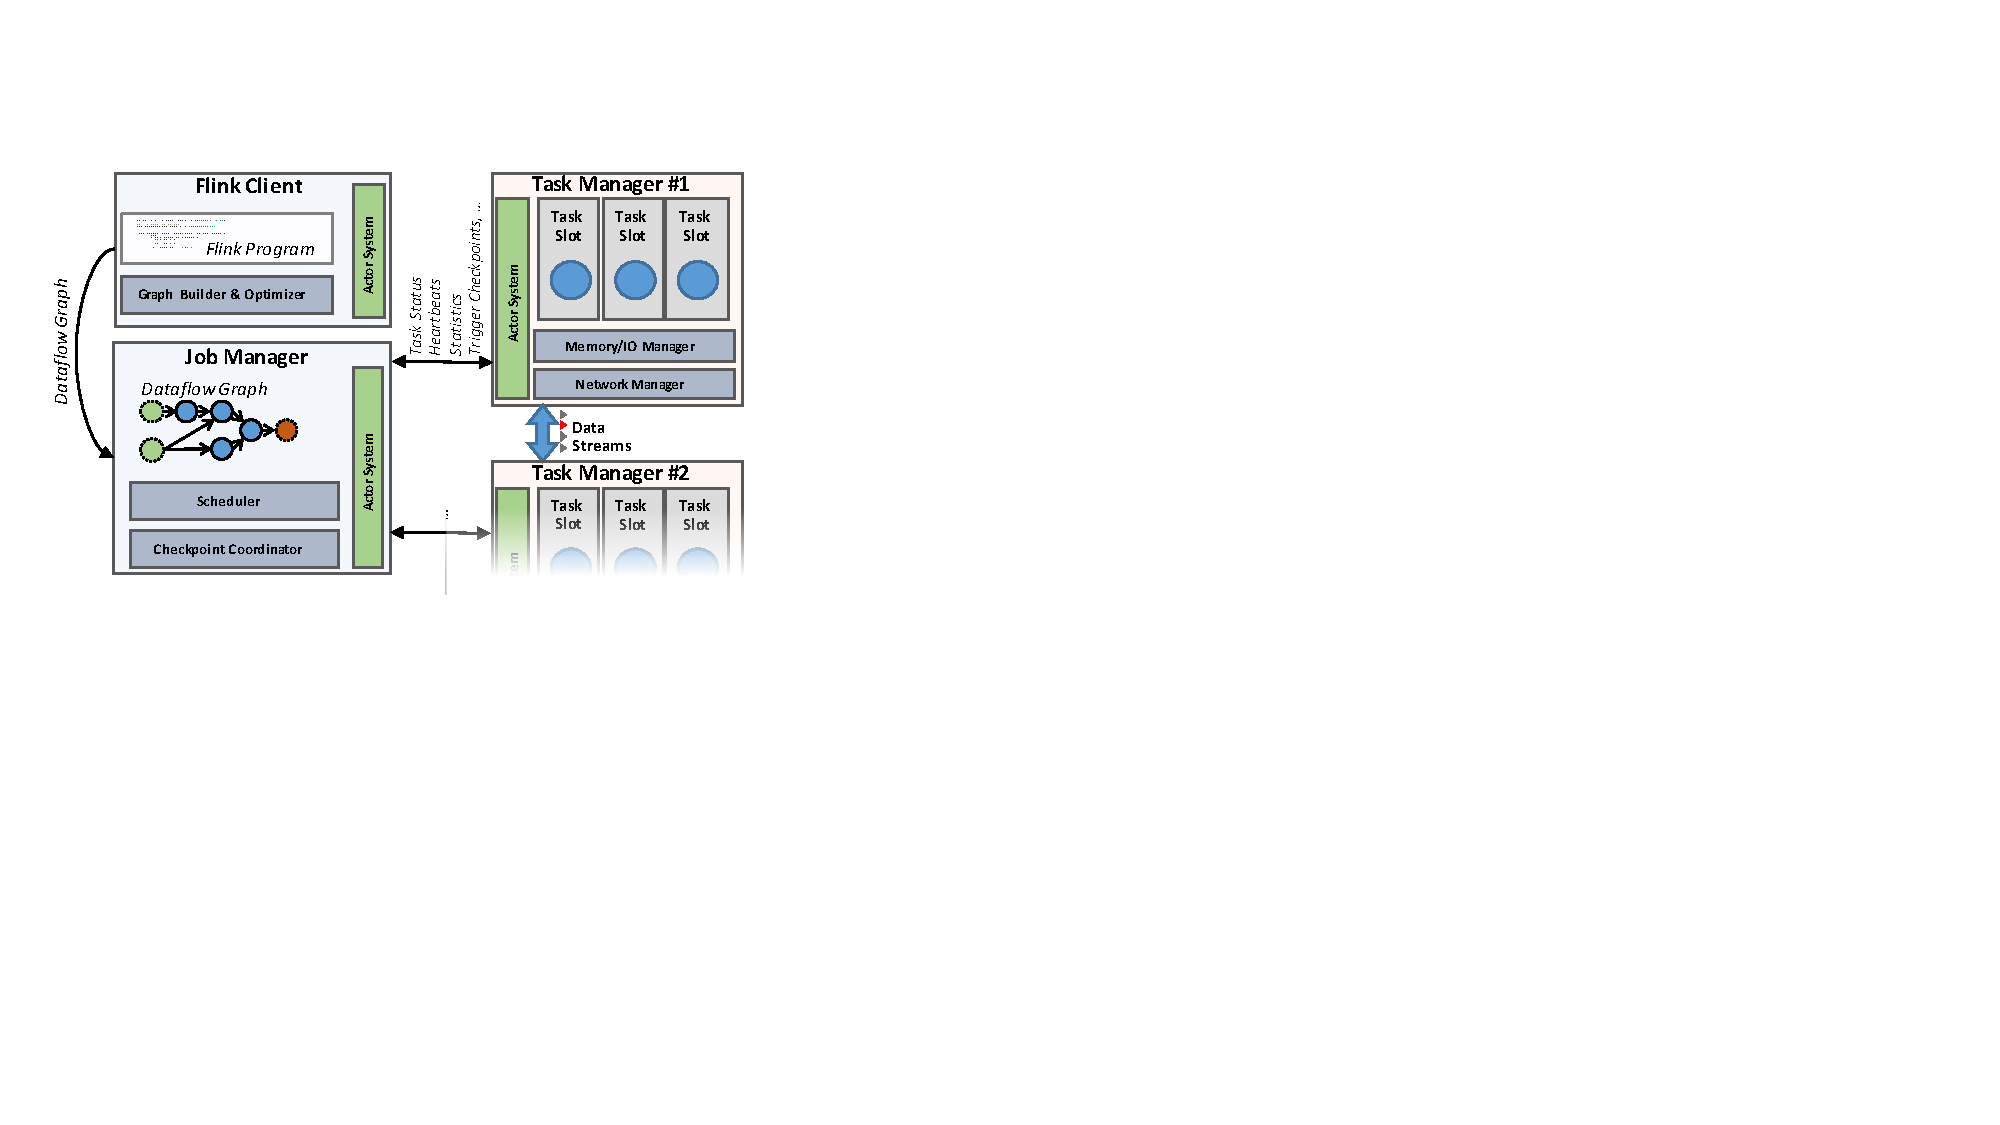
\includegraphics[width=.9\textwidth]{figs/architecture.pdf}
    \caption{Flink's Process Model.}
    \label{fig:process-model}
\end{minipage}%
\begin{minipage}{0.52\textwidth}
\centering
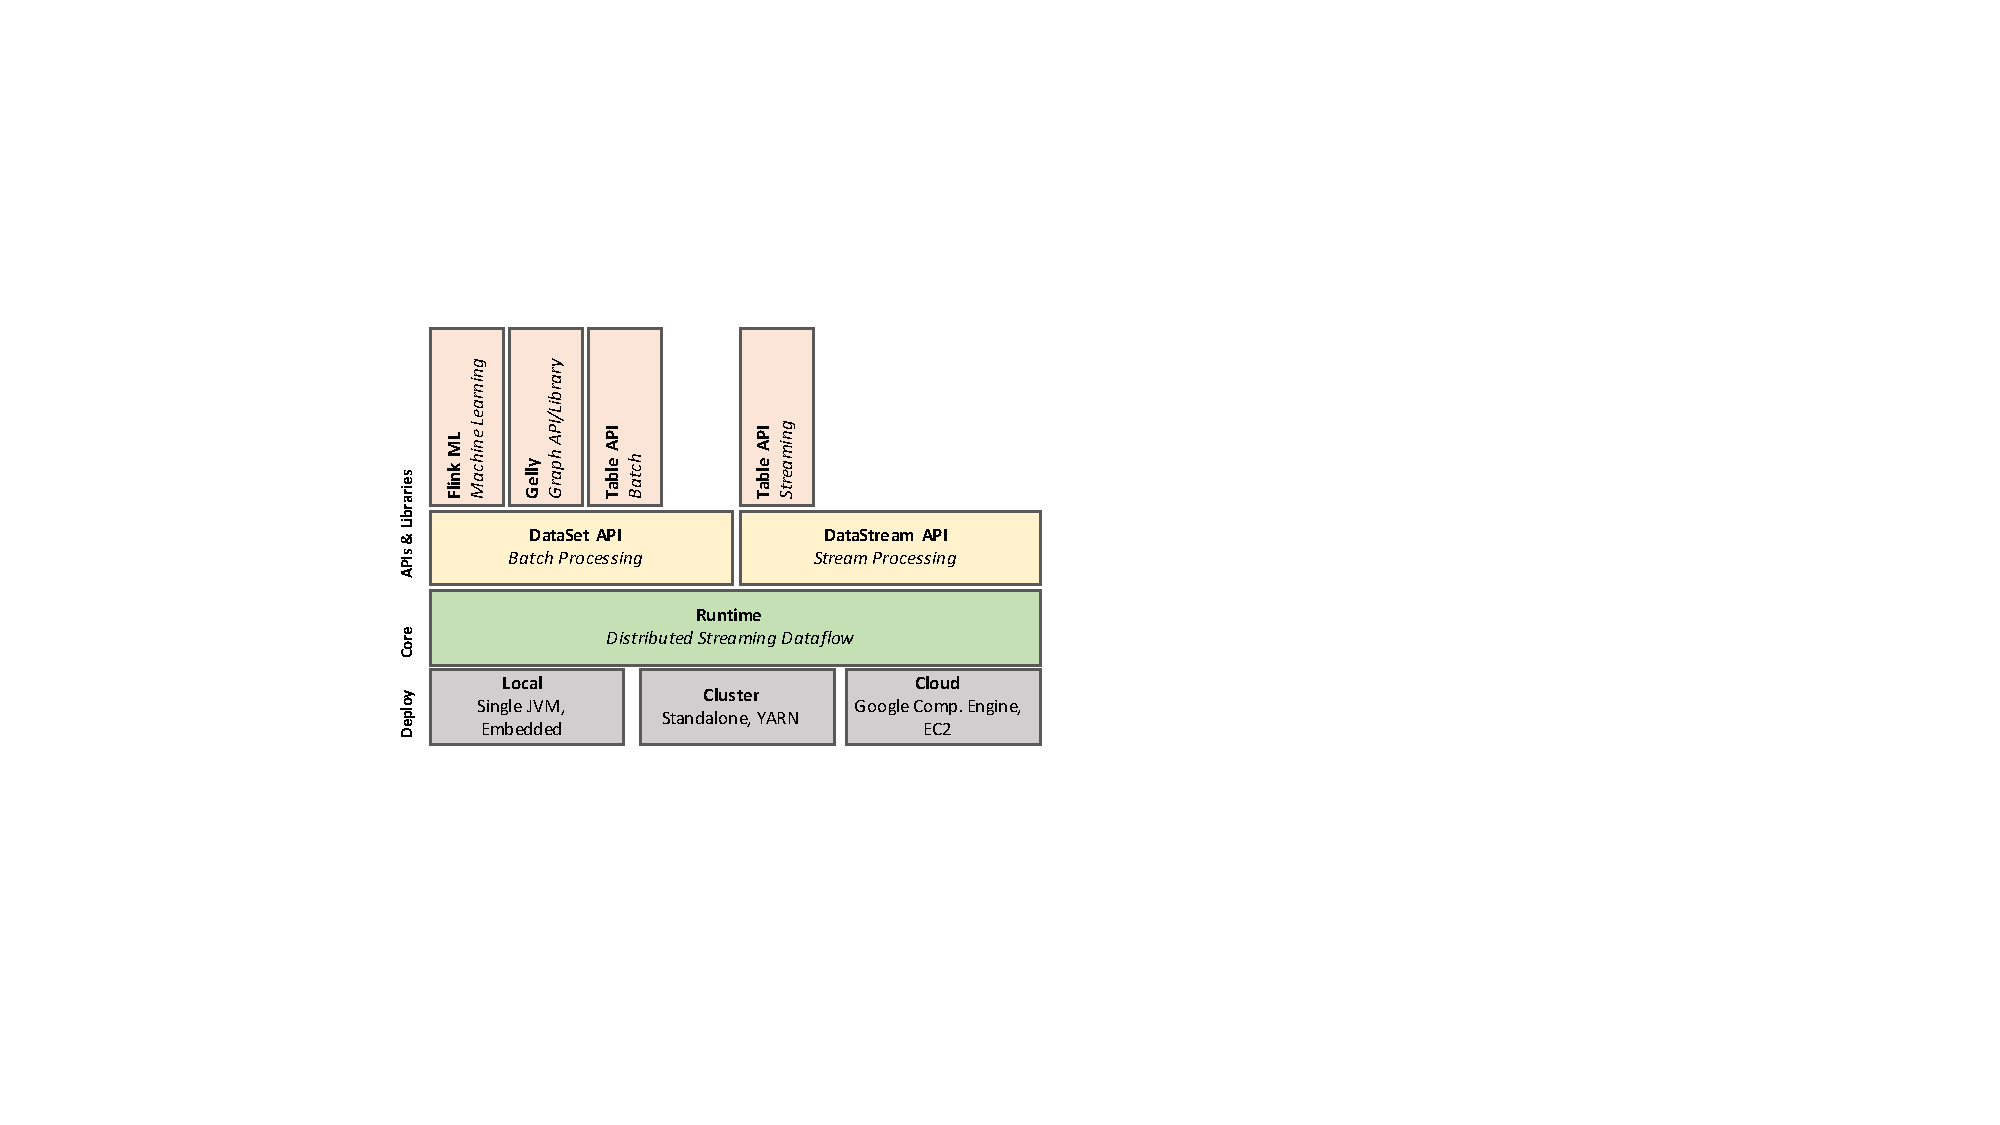
\includegraphics[width=.8\textwidth]{figs/stack.pdf}
\label{fig:FlinkStack}
\caption{Flink's Software Stack.}
\end{minipage}
\end{figure}





%!TEX root = paper.tex

\section{The Common Fabric: Streaming Dataflows}
\label{sec:execution}

Although users can write Flink programs using a multitude of APIs, all Flink programs eventually compile down to a common representation: the dataflow graph. The dataflow graph is executed by Flink's runtime engine, the common layer underneath both the batch processing (DataSet) and stream processing (DataStream) APIs.


\subsection{Dataflow Graphs}
The dataflow graph, as depicted in \autoref{fig:dataflow}, is a directed acyclic graph (DAG) that consists of (i) stateful operators, and (ii) data streams that represent data produced by an operator and are available for consumption by operators. Since dataflow graphs are executed in a data-parallel fashion, operators are parallelized into one or more parallel instances called \emph{subtasks} and streams are split into one or more \emph{stream partitions} (one partition per producing subtask). 
The stateful operators (which may be stateless as a special case) implement all processing logic, e.g., filters, hash joins, stream window functions, etc. Many of these operators are implementations of textbook versions of well known algorithms. \autoref{sec:streaming} provides details on the implementation of windowing operators. Streams distribute data between producing and consuming operators in various patterns, such as point-to-point, broadcast, re-partition, fan-out, or merge.







\begin{figure}[t!]
\begin{minipage}{1.1\linewidth}
      \centering
       \hspace{-0.1\linewidth}
      \begin{minipage}{0.55\linewidth}
        \begin{figure}[H]
        \centering
        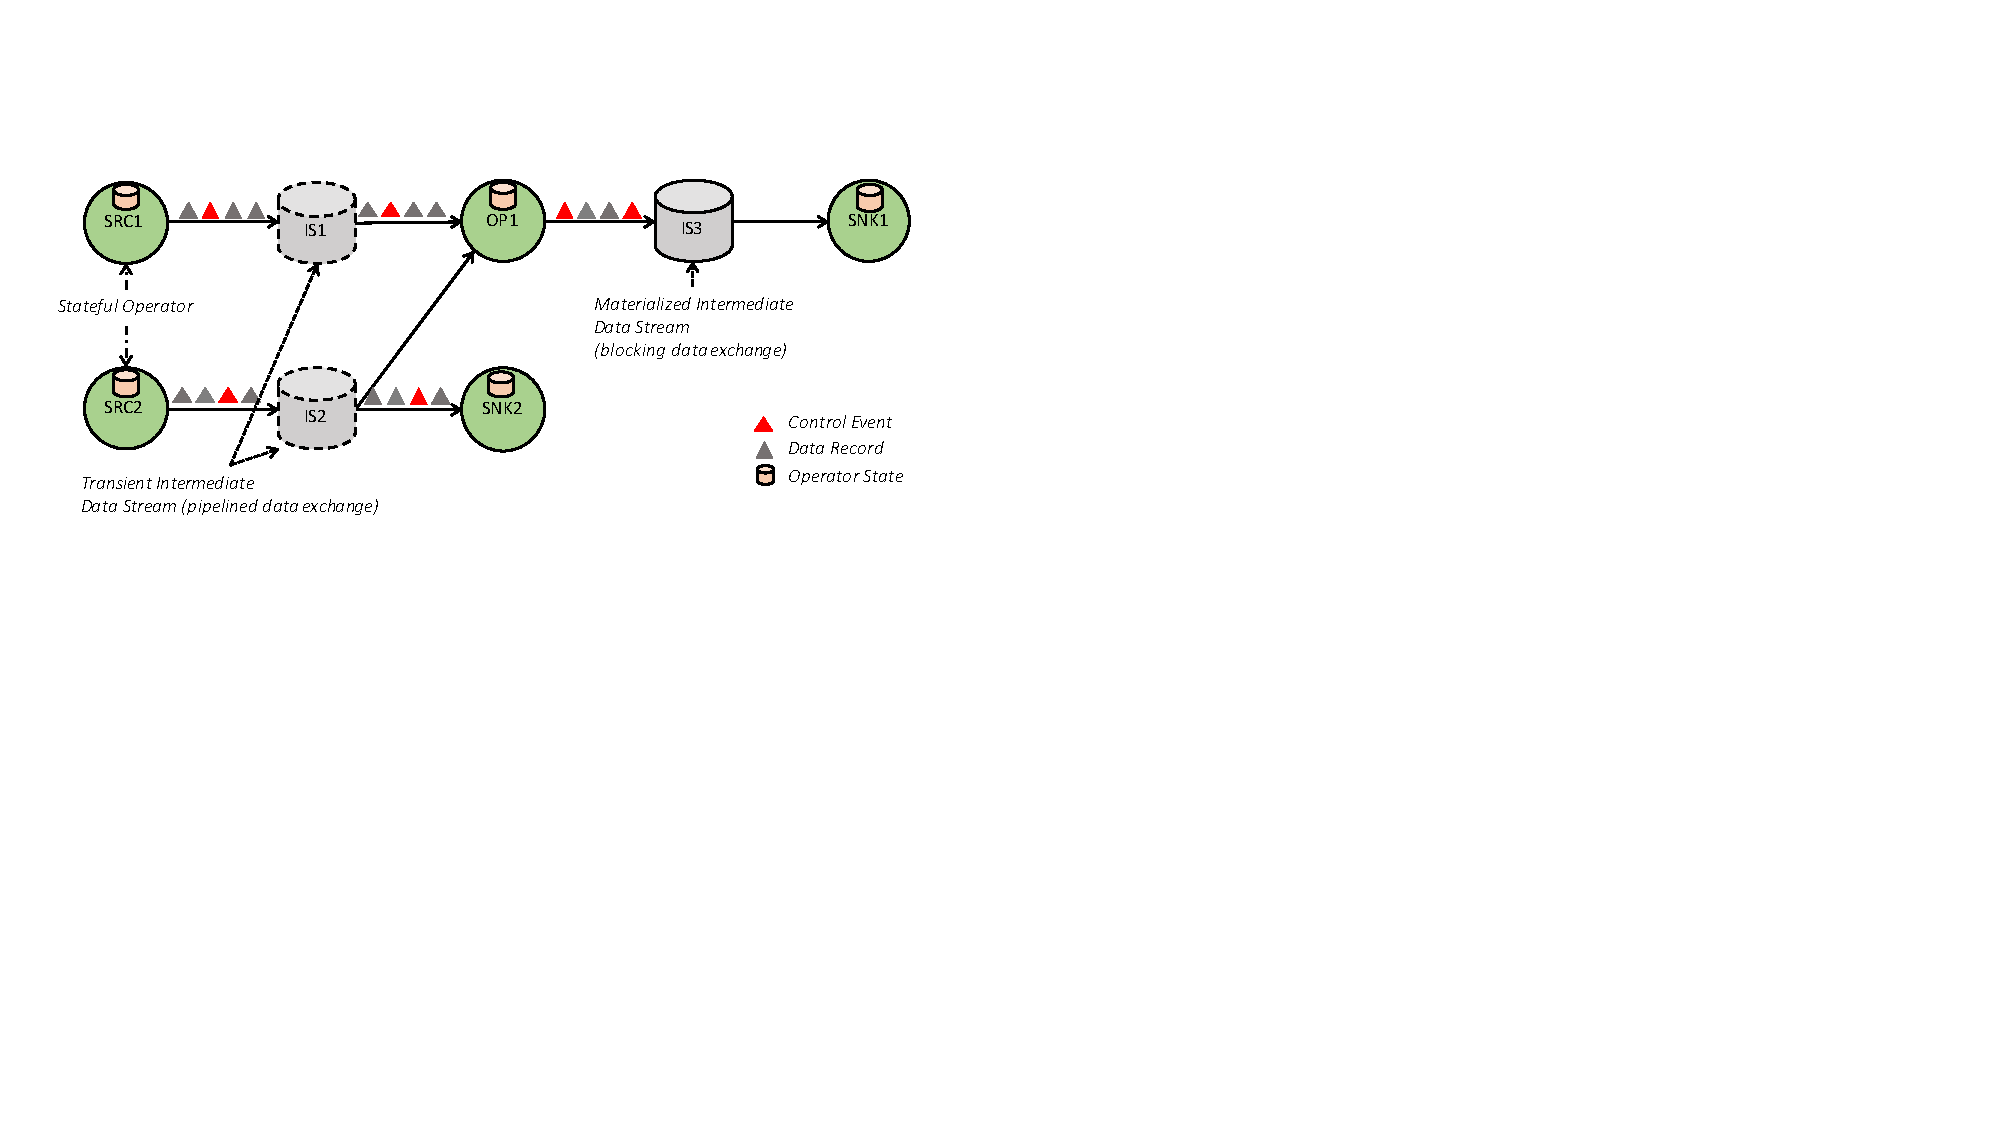
\includegraphics[width=.999\textwidth]{figs/dataflow}
        \vspace{-3mm}
        \caption{A simple dataflow graph.}
        \label{fig:dataflow}
        \end{figure}
      \end{minipage}
      \hspace{0.03\linewidth}
      % \vspace{-3mm}
      \begin{minipage}{0.32\linewidth}
          \begin{figure}[H]
				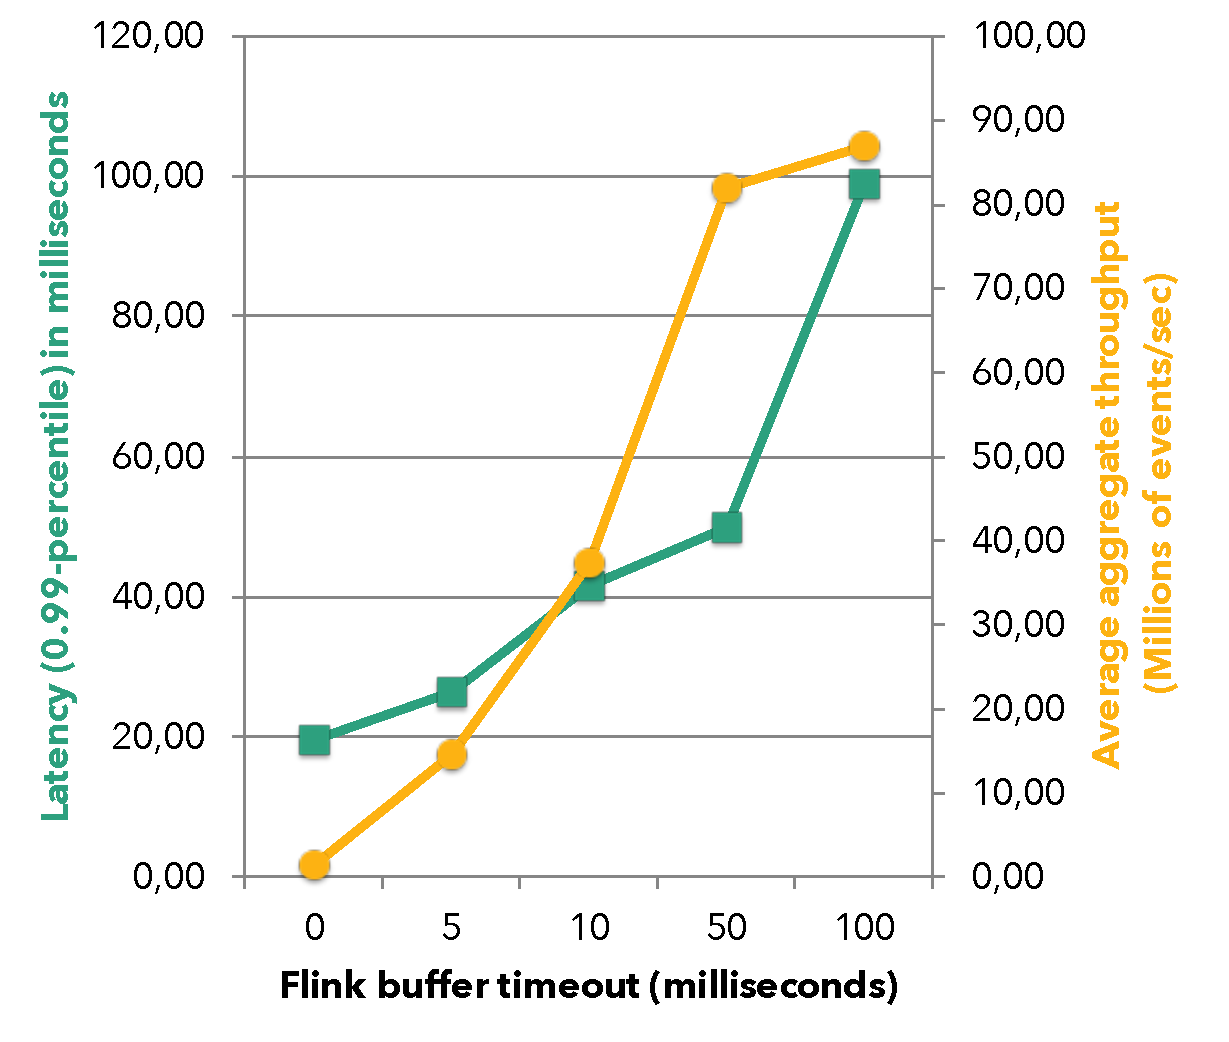
\includegraphics[width=.95\textwidth]{figs/latency-throughput.pdf}
				\vspace{-1mm}
    			\caption{The effect of buffer-timeout in latency and throughput.}
    			\label{fig:latency-throughput}
          \end{figure}
      \end{minipage}
  \end{minipage}
\end{figure}







\subsection{Data Exchange through Intermediate Data Streams}
\TODO{Asterios does not like the structure of this subsection. Minimal changes are needed but will be useful. for now it's a soup of ideas. Good news is, the content is already there.}

Flink's intermediate data streams are the core abstraction for data exchange between operators. The notion of intemediate data streams in Flink is broader than the traditional notion of a continuous transient stream. The particular behavior of a data stream is parameterized by the higher layers in Flink (e.g., the program optimizer used by the DataSet API). 


\para{Pipelined and Blocking Data Exchange.} \emph{Pipelined streams} exchange data between concurrently running producers and consumers resulting in pipelined execution. Synchronous streams propagate back pressure from consumer to producer (modulo some elasticity via intermediate buffer pools, in order to compensate for short-term throughput fluctuations). Flink uses these streams for continuous streaming programs, as well as for many parts of batch dataflows, in order to avoid materialization when possible. \emph{Blocking streams}, on the other hand, are applicable to bounded data streams. The decoupled stream buffers all of the producing operator's data before making it available for consumption, thereby separating the producing and consuming operators into different execution stages. Blocking streams naturally require more memory, frequently spill to secondary storage, and do not propagate backpressure. They are used to isolate successive operators against each other (where desired) and in situations where plans with pipeline-breaking operators such as joins, can cause distributed deadlocks.

\para{Balancing Latency and Throughput.} Flink’s data exchange mechanisms are implemented around the exchange of buffers. When a data record is ready on the producer side, it is serialized and stored into one or more buffers that can be forwarded to consumers. A buffer in Flink is sent to a consumer either i) as soon as it is full, or ii) when a timeout condition is reached. This enables Flink to achieve, high throughput by setting the size of buffers to a high value, e.g., a few kilobytes, as well as low latency by setting the buffer timeout to a low value e.g., a few milliseconds. For instance, \autoref{fig:latency-throughput} shows the effect of 

\para{Control Events.} Apart from exchanging data, streams in Flink communicate different types of control events. These are special events injected in the data stream by producing operators and are delivered in-order along with all other data records and events within a stream partition. The receiving operators react to these events by performing certain actions upon their arrival. Flink uses special types of control events such as: \vspace{-2mm}
\begin{itemize}
\item \textit{Checkpoint barriers} that coordinate checkpoints by dividing the stream into pre-checkpoint and post-checkpoint (\autoref{sec:fault-tolerance}). \vspace{-3mm}
\item \textit{Watermarks} signaling the progress of event time within a stream partition (\autoref{sec:streaming-time}). \vspace{-3mm}
\item \textit{Iteration barriers} signaling that a stream partition has reached the end of a superstep, in Bulk/Stale-Synchronous-Parallel iterative algorithms on top of cyclic dataflows (\autoref{sec:batch-iterations}). \vspace{-1mm}
\end{itemize}

Control events assume that a stream partition preserves the order of records. To this end, unary operators in Flink consuming a single stream partition, \emph{guarantee a FIFO order of records}. However, operators receiving more than one stream partition merge the streams as records arrive, in order to keep up with the streams' rate and avoid back pressure. As a result, streaming dataflows in Flink do not provide ordering guarantees after any form of repartitioning or broadcasting, and the responsibility of dealing with out-of-order records is left to the operator implementation. We found that this gives the most efficient design, as most operators do not require deterministic order (e.g., hash-joins, maps, etc.), and operators that need to compensate for out-of-order arrivals (such as event time windows) can do that more efficiently as part of the operator logic.

\subsection{Iterative Dataflows}
\TODO{Should we have a few sentences here? Would describe that cyclic flows enable iterative processing as BSP/SSP in batch [iterations paper, euranova SSP on Flink paper] and simply for streaming programs with feedback. @Stephan, could you make a start here? Just to see how you would like to see it.}

Cycles are formed by special feedback streams. Feedback streams do not act as a dependency (not treated by the scheduler, so Flink keeps simple DAG scheduling techniques) and their contents is treated as operator state (simplifies fault tolerance). 

\subsection{Fault Tolerance}

\label{sec:fault-tolerance}
Flink offers reliable execution with strict exactly-once-processing consistency guarantees and deals with failures via checkpointing and partial re-execution. The general assumption the system makes to effectively provide these guarantees is that the data sources are persistent and replayable. Examples of such sources are files and durable message queues (e.g. Apache Kafka). In practice, non-persistent sources can also be incorporated by keeping a look-ahead log within the state of the source operators.

The checkpointing mechanism of Apache Flink builds on the notion of distributed consistent snapshots/checkpoints to achieve exactly-once-processing guarantees. The possibly unbounded nature of a data stream makes re-computation upon recovery impractical, as possibly months of computation will need to be replayed considering a long running job. To bound recovery time, Flink takes a snapshot of the state of operators, including the current position of the input streams at regular intervals.

The core challenge lies in taking a consistent snapshot of all parallel operators without halting the execution of the topology. In essence, the snapshot of all operators should refer to the same logical time in the computation. The mechanism used in Flink is called Asynchronous Barrier Snapshotting, or ABS \cite{carbone2015lightweight}. Barriers are control records injected into the input streams that correspond to a logical time, and logically separate the stream to the part whose effects will be included in the current snapshot, and the part that will be snapshotted later.

\begin{figure}[t!]
	\centering
  	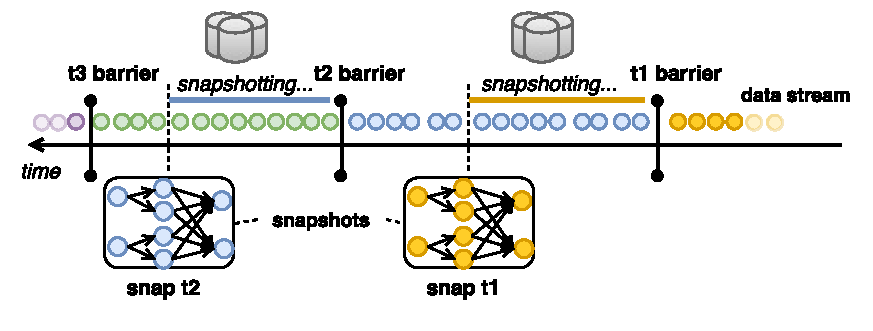
\includegraphics[width=.75\textwidth]{figs/snaps.pdf}
  	\vspace{-6mm}
	\caption{Asynchronous Barrier Snapshotting.}
	\vspace{-2mm}
	\label{fig:snapshots}
\end{figure}

An operator receives barriers from upstream and first performs an alignment phase, making sure that the barriers from all inputs have been received. Then, the operator writes its state (e.g., contents of a sliding window, or custom data structures) to durable storage (the storage backend can be an external system, e.g., HDFS). Once the state has been backed up, the operator forwards the barrier downstream. ABS bears resemblances to the seminal Chandy-Lamport algorithm for asynchronous distributed snapshots \cite{chandy1985distributed}. However, because of the DAG structure of a Flink program, ABS does not need to checkpoint in-flight records but solely rely on the aligning phase to apply all their effects to the operator states. This guarantees that the data that needs to be written to reliable storage is kept to the theoretical minimum (i.e., only the current state of the operators).

Recovery from failures reverts all operator states to their respective states taken from the last successful snapshot, and restarts the input streams starting from the latest barrier. The maximum amount of re-computation needed upon recovery is limited to the amount of input records between two consecutive barriers. Furthermore,  we note that this strategy does not eliminate the possibility for partial recovery, when upstream backup is applied.

\vspace{1mm}
\noindent ABS provides several benefits:\vspace{-3mm}
\begin{itemize}
\item It guarantees exactly-once state updates without ever pausing the computation \vspace{-3mm}
\item It is completely decoupled other forms of control messages, e.g., by events that trigger the computation of windows, thus not restricting the windowing mechanism to multiples of the checkpoint interval. \vspace{-3mm}
\item It is completely decoupled from the mechanism used for reliable storage, allowing state to be backed up to file systems, databases, etc, depending on the larger environment in which Flink is used.
\end{itemize}

% \para{The Job Graph.} Flink's execution model is based on the Job Graph, a directed acyclic graph (DAG) that consists of nodes and edges. There are two classes of nodes: (stateful) operators, and (logical) intermediate results (IRs) as presented on Figure \autoref{fig:JobGraph}. For example, the aforementioned graph consists of five operators (circles), and three intermediate results (cylinders). Operators abstract computation (e.g., transformations, joins, etc), state (e.g., a persistent counter), as well as data sources (e.g. reading data from a file system, a socket, a message queue, etc.), and data sinks. Operators produce intermediate results, as well as updates to state. An intermediate result is a logical handle (pointer) to the data that is produced by one operator. An intermediate result can be consumed by one or more operators. Intermediate results are logical in the sense that the data they point to may or may not be materialized on disk. When the JobGraph is scheduled in a cluster for execution, it is parallelized to form an ExecutionGraph that consists of tasks (parallel instances of operators), and intermediate result partitions (IRPs).


% \para{Data Transfer.} The unit of data transfer in the Flink runtime is a buffer. Buffers contain one or more records, and a record can span multiple buffers. Buffers are requested and relinquished from local buffer pools, shared among operators that live in the same task manager. An IRP is simply a collection of buffers. Work in Flink progresses (i.e., records flow through the pipeline) as long as there are buffers available, essentially implementing distributed blocking queues (the logical streams) with bounded capacity (the amount of memory available to the buffer pools, which can be configured by the user). This mechanism, in addition to implementing record network transfers doubles down as a natural way to backpressure the flow in the case of slow operators (including external systems that consume data). 

% We mentioned that the intermediate results are logical handles to the data, rather than the data itself. Internally, intermediate results are abstract classes with many implementations. These implementations can perform pipelined data exchange, and blocking data exchange.

% \para{Pipelined Data Exchange.} Pipelining (also called intra-operator parallelism), means that a producing and a consuming operator make progress at the same time, without the consumer waiting for the producer to finish. Pipelining is required in streaming systems, and is also used in batch systems to reduce latency. Flink implements pipelining by implementing intermediate results which activate network transfers between the producer task and consumer task,  as soon as their first buffer is available. Flink allows the configuration of its buffers' size and timeout. A buffer is sent to its consumer task as soon it is filled,  or as soon as a timeout is reached. Hence, by setting the buffer size and/or timeout to lower values, one can reduce latency, while achieving the opposite effect (i.e., high throughput) by using higher values.

% \para{Blocking Data Exchange.} Sometimes it is desirable to break a job into stages, scheduling and executing each stage individually (e.g., to enable interactive processing, and better staging of resources in large batch jobs). To do that, the system has to materialize intermediate results (in memory or disk). Flink implements blocking data exchange via an intermediate result that signals its availability only when all the buffers from the producer have been materialized. The cached buffers can double down as a materialized reusable intermediate result. 


%!TEX root = paper.tex

\section{Stream Analytics on Top of Dataflows}
\label{sec:streaming}


Flink’s DataStream API implements a full stream analytics framework on top of Flink’s runtime, including the mechanisms to manage time (including out-of-order event processing), defining windows, and maintaining and updating user-defined state. The streaming API is based on the notion of a DataStream, a (possibly unbounded) immutable collection of elements of a given type. Since Flink’s runtime already supports pipelined data transfers, continuous stateful operators, and a fault tolerance mechanism for consistent state updates, overlaying a stream processor on top of it, essentially boils down to implementing a windowing system and a state interface. As noted, these are invisible to the runtime, which sees windows as just an implementation of stateful operators. 

\subsection{The Notion of Time}
\label{sec:streaming-time}
Flink distinguishes between two notions of time: i) event time, that  stands for the time that an event was generated at its origin (e.g., the time that a sensor or a mobile device generated a signal) and ii) processing time, that is the wall-clock time of the machine that is processing the data.

In distributed systems there is an arbitrary skew between event-time and processing-time \cite{akidau2015dataflow}. This may mean arbitrary delays for getting an answer based on event-time semantics. To avoid arbitrary delays these systems regularly insert special events called ‘low watermarks’ that mark a global progress measure. In the case of time progress for example, that includes a time attribute ‘t’ indicating that all events lower than ‘t’ have already entered an operator. The watermarks aid the execution engine to process events in the correct event order and serialize operations (such as window computations) via a unified measure of progress.

Watermarks originate at the sources of a topology, where we can determine the time inherent in future elements. The watermarks propagate from the sources throughout the other operators of the data flow. Operators decide how they react to watermarks. Simple operations such as map/filter just forward the watermarks they receive, while more complex operators that do calculation based on the watermarks (e.g., event time windows) first compute results triggered by a watermark and then forward it. If an operation has more than one input, the system only forwards the minimum of the incoming watermarks to the operator, ensuring correct results. 

Flink programs that are based on processing time, rely on the machine clocks, and hence a less reliable notion of time, but exhibit lower latency. Programs that are based on event time provide the most reliable semantics, but may exhibit latency due to event time-processing time lag. Flink includes a third notion of time as a special case of event time called ingestion time, which is the time that events enter Flink. This provides  lower processing latency than event time, and more accurate results compared to processing time.


\subsection{Stream Discretization}
Many incremental computations over unbounded streams are often evaluated over finite logical views, called windows. Apache Flink creates windows via a highly flexible discretization process which is composed out of three core functions: a window assigner and optionally a trigger and an evictor. All three functions can be selected among a pool of common predefined implementations (e.g. sliding time window) or explicitly defined by the user (via UDFs).

More specifically, the assigner is responsible for assigning each record to logical windows. For example, this decision can be based on the timestamp of a record when it comes to event-time discretization. Note that in the case of sliding windows, an element can belong to multiple logical windows. An optional trigger defines when the operation associated with the window definition is performed. Finally, an optional evictor determines which records to retain within each window. The discretization operation of Apache Flink is uniquely capable of covering all known window types such as periodic time/count-windows, punctuation, landmark, session and delta windows. Note that windows incorporate out-of-order processing seamlessly as in \cite{li2005semantics, akidau2015dataflow} and, in principle, subsumes these discretization models. For example, below is a window definition of 6 seconds that slides every 2 seconds (Assigner). The window results are computed once the watermark passes the end of the window (Trigger).

\begin{lstlisting}[language=Java]
stream
  .window(SlidingTimeWindows.of(Time.of(6, SECONDS), Time.of(2, SECONDS))
  .trigger(EventTimeTrigger.create())
\end{lstlisting}

A global window creates a single logical group. The following example defines a global window (assigner) that invokes the operation on every 1000 events (trigger) while keeping the last 100 elements (evictor). 

\begin{lstlisting}[language=Java]
stream
  .window(GlobalWindow.create())
  .trigger(Count.of(1000))
  .evict(Count.of(100))
\end{lstlisting}

Note that streams are already partitioned on a key before windowing, so the above is a local operator that does not require coordination between machines. This mechanism can be used to implement a wide variety of windowing functionality \cite{akidau2015dataflow}. 


\subsection{Stateful Stream Processing}
\TODO{Asterios: This is very developer-heavy. We need to show the big picture. Long story short, the side-effect free functional view of the system changes with mutable state that is managed by the system. Why do we need state? What can be state? How is it implemented in Flink. @Paris, please answer these 3 questions in 2-3 paragraphs. The example below could also be missing.}

Simple programs in Flink’s DataStream API look like functional, side effect-free programs consisting of transformations on unbounded immutable collections. However, to cover the need for stateful operations, we incorporate explicit mutable state in the API by providing: $i)$ Operator interfaces or annotations to statically register explicit local variables within the scope of an operation;  $ii)$ an OperatorState abstraction for marking partionable dynamic state and its operations.  Flink’s checkpointing mechanism guarantees that any registered state is durably accessed exactly-once per operation via checkpointing. 

As an example consider a stream wordNums containing words and an associated number for each word. We can use the partitionable  OperatorState in a stateful map function to compute a rolling average number seen per word by marking a sum and count per word as explicit states along with their updates:

\begin{lstlisting}[language=Java]
wordNums.keyBy(0).map(new StatefulAverage()) 

public class StatefulAverage implements RichMapFunction<Long, Double> {
    private OperatorState<Long> sum;
    private OperatorState<Long> count;

    public Double reduce(Tuple2<String,Long> num) {
        count.update(count.value() + 1);
        sum.update(sum.value() + num.f1)
        return new Tuple2(num.f0, (double) sum.value()/count.value());
    }
...
}
\end{lstlisting}

\subsection{Fault Tolerance via Asynchronous Snapshots}
\label{sec:fault-tolerance}
The fault tolerance mechanism of Apache Flink for unbounded streams builds on the notion of distributed consistent snapshots/checkpoints to achieve exactly-once-processing guarantees. The possibly unbounded nature of a data stream in the model of the DataStream API makes recomputation upon recovery impractical, as possibly months of computation will need to be replayed considering a long running job. To bound recovery time, Flink takes a snapshot of the state of operators, including the current position of the input streams at regular intervals.

The core challenge lies in taking a consistent snapshot of all parallel operators without halting the execution of the topology. In essence, the snapshot of all operators should refer to the same logical time in the computation. The mechanism used in Flink is called Asynchronous Barrier Snapshotting, or ABS \cite{carbone2015lightweight}. Barriers are control records injected into the input streams that correspond to a logical time, and logically separate the stream to the part whose effects will be included in the current snapshot, and the part that will be snapshotted later.

\begin{figure}[ht]
	\centering  	
  	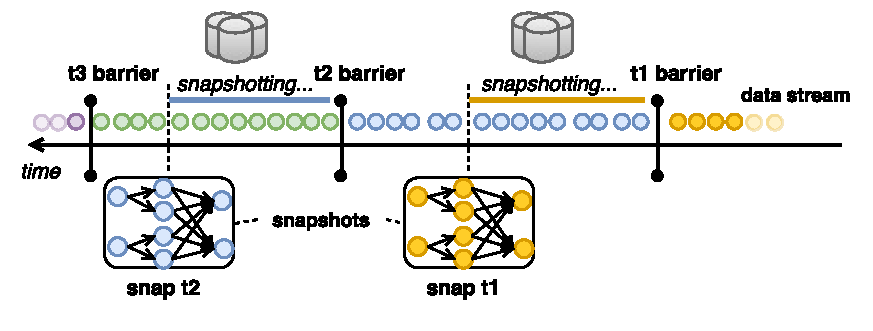
\includegraphics[width=.75\textwidth]{figs/snaps.pdf}
  	\vspace{-6mm}
	\caption{Asynchronous Barrier Snapshotting.}
	\vspace{-2mm}
	\label{fig:snapshots}
\end{figure}

An operator receives barriers from upstream and first performs an alignment phase, making sure that the barriers from all inputs have been received. Then, the operator writes its state (e.g., contents of a sliding window, or custom data structures) to durable storage (the storage backend can be an external system, e.g., HDFS). Once the state has been backed up, the operator forwards the barrier downstream. ABS bears resemblances to the seminal Chandy-Lamport algorithm for asynchronous distributed snapshots \cite{chandy1985distributed}. However, because of the DAG structure of a Flink program, ABS does not need to checkpoint in-flight records but solely rely on the aligning phase to apply all their effects to the operator states. This guarantees that the data that needs to be written to reliable storage is kept to the theoretical minimum (i.e., only the current state of the operators).

Recovery from failures reverts all operator states to their respective states taken from the last successful snapshot, and restarts the input streams starting from the latest barrier. The maximum amount of re-computation needed upon recovery is limited to the amount of input records between two consecutive barriers. Furthermore,  we note that this strategy does not eliminate the possibility for partial recovery, when upstream backup is applied.



\vspace{1mm}
\noindent ABS provides several benefits:\vspace{-3mm}
\begin{itemize}
\item It guarantees exactly-once state updates without ever pausing the computation \vspace{-3mm}
\item It is completely decoupled other forms of control messages, e.g., by events that trigger the computation of windows, thus not restricting the windowing mechanism to multiples of the checkpoint interval. \vspace{-3mm}
\item It is completely decoupled from the mechanism used for reliable storage, allowing state to be backed up to file systems, databases, etc, depending on the larger environment in which Flink is used.
\end{itemize}




%!TEX root = paper.tex

\section{Batch analytics on top of dataflows}
\label{sec:batch}
A bounded data set is a special case of an unbounded data stream. Thus, a streaming program that inserts all of its input data in a window can form a ``batch`` program and ``batch analytics``, or ``batch processing`` should be fully covered by Flink's features that we presented above. However, \begin{inparaenum}[i)]
  \item the syntax, i.e., the API for batch computation can be simplified (not need for window definitions, simpler joins and loops),
  \item we can simplify the fault tolerance mechanisms and
  \item we can apply query optimization borrowing ideas from MPP database systems.
\end{inparaenum}
For these reasons, Flink treats specially batch computations, by implementing the above optimizations. For enabling batch computations on top of it's streaming runtime, Flink embeds blocking versions of its operators (sorts, joins, etc) within its runtime. These operators simply block until they have received all of their input. Moreover, Flink currently disables the asynchronous snapshotting mechanism for batch programs, and simply uses backtracking based recovery as first described in Dryad.~\cite{isard2007dryad}

With these established, we look that the batch-specific optimizations mentioned above: query optimization, and query processing on paged (managed) memory.

\para{Query Optimization.} Flink's optimizer builds on techniques from parallel database systems such as plan equivalences, cost models and interesting properties. However, the arbitrary UDF-heavy DAGs that make up Flink's dataflow programs, do not allow a traditional optimizer to employ database techniques out of the box [black-boxes], since the operators hide their semantics from the optimizer. For the same reason, cardinality and cost estimation methods are equally difficult to employ. Flink's optimizer employs a number of novel methods for overcoming these issues~\cite{blackBoxes, stratosphere, DBLP:journals/pvldb/EwenTKM12} for which we provide a short overview below. Flink's runtime supports various execution strategies including repartition/broadcast data transfer, as well as sort-based grouping and sort- and hash-based join implementations. Flink's optimizer enumerates different physical plans based on the concept of interesting properties propagation~\cite{scopeOptimizer}, using a cost-based approach to choose among multiple physical plans. The cost includes network/disk I/O and CPU cost. To overcome the cardinality estimation issues that were mentioned earlier, Flink's optimizer uses hints that are provided by the programmer.

\para{Memory Management.} Building on database technology, Flink, instead of storing objects in the JVM's heap, serializes objects into a  memory segments. These memory segments resemble database blocks into which, Java objects representing the tuples that go through the runtime are serialized. Operations such as sorting, and joining, operate as much as possible on the binary data, keeping the de/serialization overhead at a minimum and partially spilling data to disk when needed. To handle arbitrary objects, Flink uses type inference, and  custom serialization mechanisms.  By keeping the data processing on binary representation and off-heap, Flink manages to reduce the garbage collection overhead, and implement cache-efficient and robust algorithms that scale gracefully in under memory constraints.

\para{Native Iterations on top of Dataflows.} The final aspect of Flink on which we focus, is how to implement loops on top of the Flink's dataflow engine. Some approaches execute iterations by submitting new jobs for each iteration or by adding additional nodes to a running DAG~\cite{DBLP:journals/pvldb/BuHBE10, DBLP:conf/hotcloud/ZahariaCFSS10}, hiding from  the engine that it is executing an iterative program. The approach, implemented in Naiad~\cite{murray2013naiad} adds feedback edges in the dataflow graph, supporting graphs with cycles, that  allow for nested iterations. A third approach was to design specialized engines around iterative processing along (e.g., Apache Giraph, and GraphLab) allowing to reduce the number of computations in each iteration.~\cite{low2012distributed}

Flink follows an approach that maintains the DAG-based runtime, but allows for special ``head'' and ``tail'' tasks to signify the beginning and end of iteration, that exchange data via shared memory. This approach simulates a cyclic dataflow within a DAG engine making Flink competitive with specialized graph engines [], while outperforming the driver-based approach []. Flink supports delta iterations [], which exploit sparse computational dependencies, and are used, as the basis for Gelly, Flink's Graph API. Finally, Flink offers Bulk Synchronous Parallel (BSP) iterations in its DataSet API, and asynchronous iterations in its DataStream API.

%!TEX root = paper.tex

\section{Related work}
\label{sec:related}
There is, by now, a wealth of engines for distributed batch and stream analytical processing. We categorise these systems below. 

\para{Batch Processing.} Apache Hadoop~\cite{CUSTOM:web/Hadoop} is the most popular open source system for large-scale data analysis that is based on the MapReduce paradigm~\cite{DBLP:journals/cacm/DeanG08}. Dryad~\cite{isard2007dryad}, introduced embedded user-defined functions in general DAG-based dataflows and was used by SCOPE~\cite{scopeOptimizer} which added a language and an SQL optimizer on top of it. Apache Tez~\cite{CUSTOM:web/Tez} can be seen as an open source implementation of the ideas proposed in Dryad. MPP databases [], and recent open-source implementations~\cite{CUSTOM:web/Drill} [Impala] restrict their API to SQL variants. Very similar to Flink, Apache Spark~\cite{CUSTOM:web/Spark} is a very popular data processing framework that implements a DAG-based processing framework, provides an SQL optimizer, performs driver-based iterations, and treats stream computations as micro-batches. In contrast, Flink is the only system that
\begin{inparaenum}[i)]
  \item supports an optimizer that can optimize DAG programs beyond SQL queries,
  \item is able to perform very efficient iterative processing natively,
  \item includes stream processing as a first-class citizen, enabling more complex use cases than micro-batches.
\end{inparaenum}

\para{Stream Processing.} There is a wealth of work on streaming systems, that includes commercial systems like StreamBase, Microsoft StreamInsight, and IBM InfoSphere Streams. Many of these systems are based on research in the database community in projects such as Telegraph [], Aurora/Borealis~\cite{abadi2005design}, Stanford STREAM~\cite{arasu2004stream}, Trill~\cite{chandramouli2014trill} and IBM System S~\cite{chandramouli2014trill}. Most of the above systems are either
\begin{inparaenum}[i)]
  \item academic prototypes,
  \item closed-source commercial products,
  \item do not scale the computation horizontally on clusters of commodity servers.
\end{inparaenum}
Newer open source streaming systems that scale horizontally, such as Apache Storm~\cite{CUSTOM:web/Storm} and Apache Samza~\cite{CUSTOM:web/Samza}, provide low level APIs and offer only at-least-once and at-most-once guarantees. MillWheel~\cite{akidau2013millwheel}, a closed-source system at Google provides exactly-once guarantees with low latency and is used by Google Dataflow~\cite{akidau2015dataflow} to implement  out-of-order stream analytics. To the best of our knowledge, Flink is the only open-source project that
\begin{inparaenum}[i)]
  \item offers high level APIs and processing libraries,
  \item provides state management with exactly-once guarantees and
  \item achieves high throughput and low latency, serving both batch and true streaming computations equally well.
\end{inparaenum}

\section{Conclusion}
\label{sec:conclusions}
In this paper we presented Apache Flink, a platform that implements a universal dataflow engine designed to perform both stream and batch analytics. Flink's dataflow engine treats operator state and logical intermediate results as first class citizens, and is used by both the batch and a data stream APIs, with different parameters. The streaming API that is built on top of  Flink's streaming dataflow engine, provides the means to keep recoverable state and to partition, transform, and aggregate windows of a data stream. While batch computations are, in theory, a special case of a streaming computations, Flink treats them specially, by optimizing their execution with a novel query optimizer, and by implementing blocking operators that gracefully spill to disk in the absence of memory. 
{
\small
\bibliographystyle{abbrv}
\bibliography{references}
}
\end{document}